\documentclass[11pt,a4paper]{article}
\usepackage[spanish,activeacute]{babel}
\decimalpoint
\usepackage[utf8]{inputenc}
\usepackage{listingsutf8}
\usepackage{amsmath}
\usepackage{amsfonts}
\usepackage{amssymb}
\usepackage{graphicx}
\usepackage{color}
\usepackage{listings}
\usepackage{amsthm}
\usepackage{caption}
\usepackage{subcaption}
\usepackage{dsfont}
\usepackage{comment}
\usepackage{enumerate}
\usepackage{mathtools,xparse}
\usepackage{ mathrsfs }
\usepackage{float}
\usepackage{listings}
\usepackage{xcolor}
\usepackage{esvect}
%% CODIGO PYTHON
\definecolor{codegreen}{rgb}{0,0.6,0}
\definecolor{codegray}{rgb}{0.5,0.5,0.5}
\definecolor{codepurple}{rgb}{0.58,0,0.82}
\definecolor{backcolour}{rgb}{0.93,0.93,0.93}

\lstdefinestyle{mystyle}{
    backgroundcolor=\color{backcolour},   
    commentstyle=\color{codegreen},
    keywordstyle=\color{magenta},
    numberstyle=\tiny\color{codegray},
    stringstyle=\color{codepurple},
    basicstyle=\ttfamily\footnotesize,
    breakatwhitespace=false,         
    breaklines=true,                 
    captionpos=b,                    
    keepspaces=true,                 
    numbers=left,                    
    numbersep=5pt,                  
    showspaces=false,                
    showstringspaces=false,
    showtabs=false,                  
    tabsize=2
}

\lstset{style=mystyle, inputencoding=utf8, extendedchars=true, literate={á}{{\'a}}1 {ó}{{\'o}}1 {é}{{\'e}}1 {ú}{{\'u}}1 {í}{{\'i}}1 {ñ}{{\~n}}1,}
%CODIGO PYTHON
\usepackage[left=2.33cm, right=2.31cm, top=2.42cm, bottom=2.42cm]{geometry}
%\renewcommand{\rmdefault}{mathpazo}
%\usepackage{mathpazo}

\usepackage[]{hyperref}
\hypersetup{
    pdftitle={Práctica 2 - AA},
    pdfauthor={Grupo 6},
    pdfsubject={ },
    pdfkeywords={keyword1, keyword2},
    bookmarksnumbered=true,     
    bookmarksopen=true,         
    bookmarksopenlevel=1,       
    colorlinks=true,   
    linkcolor=black,         
    pdfstartview=Fit,           
    pdfpagemode=UseOutlines,
    pdfpagelayout=TwoPageRight
}


\DeclarePairedDelimiter{\norm}{\lVert}{\rVert}
\NewDocumentCommand{\normL}{ s O{} m }{%
  \IfBooleanTF{#1}{\norm*{#3}}{\norm[#2]{#3}}_{L_2(\Omega)}%
}
\newtheorem{theorem}{Teorema}

\theoremstyle{definition}
\newtheorem{definition}{Definición}[section]


\newtheorem{proposition}{Proposición}[section]


\newtheorem{corolary}{Corolario}[section]


\newtheorem{lema}{Lema}[section]

	\newcommand{\R}{\mathbb{R}}
	\newcommand{\N}{\mathbb{N}}
	\newcommand{\C}{\mathbb{C}}


\title{
\normalfont \normalsize 
\textsc{\small APRENDIZAJE AUTOMÁTICO} \\ [10pt]
	
	
\huge \bf Práctica 2\\


	}

\author{Mario Muñoz Mesa}
\date{20 de mayo de 2021}

\begin{document}

	\maketitle
	\renewcommand*\contentsname{Índice}	
	\tableofcontents
	
	\newpage
	

	\section{Ejercicio sobre la complejidad de H y el ruido.}
	\subsection{Apartado 1}
	%Vamos a dibujar gráfica de nube de 50 puntos siguiendo distribución uniforme en $[-50, 50]\times [-50,50]$
	Suponemos vector aleatorio $\mathbf{x}=(x_1, x_2)$ con $x_1 \sim U(-50,50)$, $x_2 \sim U(-50,50)$, esto es, las distribuciones de probabilidad que inducen $x_1$ y $x_2$ siguen una distribución uniforme $U(-50,50)$, es decir, una distribución con función de densidad
	$$f(x)=\frac{1}{50-(-50)}=\frac{1}{100} \quad \forall x \in [-50,50]$$
	donde encontrar valores en intervalos de $[-50,50]$ de igual longitud es equiprobable.
	\iffalse donde la probabilidad de encontrar valor en un intervalo $I\subseteq [-50,50]$ depende únicamente de la longitud de $I$ y no de la posición de $I$ en $[-50,50]$. $(a, a+r)\subseteq $\fi \\Generamos realización muestral $\mathbf{x}_1,\ldots, \mathbf{x}_{50}$ mediante \texttt{simula\_unif(50, 2, [-50,50])}, aquí cada $\mathbf{x}_i$ con $i\in \{1,\ldots,50\}$ es una dupla. Mostramos la gráfica generada:
	\begin{figure}[H]
		\centering
		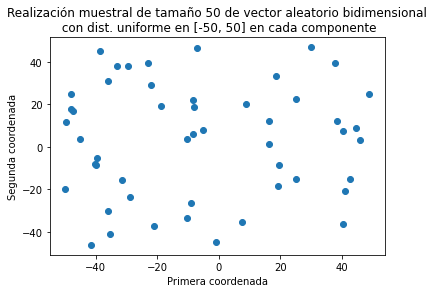
\includegraphics[width=0.6\textwidth]{images/dist_50_uniforme}
		\caption{Realización muestral de tamaño 50 de vector aleatorio bidimensional con distribución uniforme $U(-50,50)$ en cada componente. Realización generada mediante \texttt{simula\_unif(50, 2, [-50,50])}}
	\end{figure}
	
	%Vamos a dibujar gráfica de 50 puntos siguiendo distribución gaussiana (distribución normal) $N((0,0), (5,7))$ 
	Suponemos ahora vector aleatorio $\mathbf{x}=(x_1,x_2)$ con $x_1 \sim N(0,5)$, $x_2 \sim N(0,7)$, esto es, la distribución de probabilidad que induce $x_1$ es una distribución normal con media 0 y varianza 5, y la distribución de probabilidad que induce $x_2$ es una distribución normal con media 0 y varianza 7. Las funciones de densidad de $x_1$ y $x_2$ son
	$$f_1(x)= \frac{1}{\sqrt{5}\sqrt{2\pi}}e^{-\frac{x^2}{10}}\quad \forall x \in \R, \quad f_2(x)= \frac{1}{\sqrt{7}\sqrt{2\pi}}e^{-\frac{x^2}{14}} \quad \forall x \in \R$$ respectivamente.\\
	Para el caso de $x_2$ tenemos una distribución con más dispersión ya que tiene varianza 7, mientras que para $x_1$ tenemos varianza 5.\\
	 Generamos realización muestral $\mathbf{x}_1,\ldots, \mathbf{x}_{50}$ mediante \texttt{simula\_gaus(50, 2, np.array([5,7]))}, aquí cada $\mathbf{x}_i$ con $i\in \{1,\ldots,50\}$ es una dupla. Mostramos la gráfica generada:
	\begin{figure}[H]
		\centering
		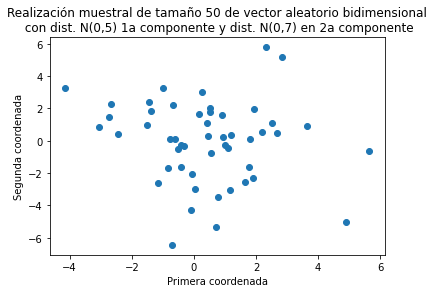
\includegraphics[width=0.62\textwidth]{images/dist_50_gaussiana}
		\caption{Realización muestral de tamaño 50 de vector aleatorio bidimensional con distribución $N(0,5)$ en primera componente y distribución $N(0,7)$ en segunda componente. Realización generada mediante \texttt{simula\_gaus(50, 2, np.array([5,7]))}}
	\end{figure}
	Podemos observar un cambio significativo de escala respecto a la anterior gráfica debido a las ``bajas'' varianzas 5 y 7.
	\subsection{Apartado 2}
	De nuevo, si $\mathbf{x}=(x_1,x_2)$ vector aleatorio con $x_1 \sim U(-50,50)$, $x_2 \sim U(-50,50)$; generamos realización muestral $\mathbf{x}_1,\ldots, \mathbf{x}_{100}$ mediante \texttt{simula\_unif(100, 2, [-50,50])}, aquí cada $\mathbf{x}_i$ con $i\in \{1,\ldots,100\}$ es una dupla.
	
	Simulamos recta con \texttt{simula\_recta([-50, 50])}, quedándonos la función $f$ que define la frontera de clasificación 
	$$f(x,y)=y-(\underbrace{-0.6771584922002485}_a x + (\underbrace{-18.89022818933684}_b))$$% y obtenemos $a=-0.6771584922002485$, $b=-18.89022818933684$
	la recta que obtuvimos es $ax+b$. Dado un punto $(\tilde x, \tilde y)$,
	$$signo(f(\tilde x,\tilde y))=\begin{cases} +1 & \text{ si } (\hat x,\hat y) \text{ está por encima de la recta}\\ -1 & \text{ si } (\hat x, \hat y) \text{ está por debajo de la recta} \end{cases}$$ 
	Después de clasificar la muestra con $signo(f(x,y))$ obtenemos la gráfica
	\textit{Nota:} en el código la función que clasifica la llamamos $f$ y ya incluye la función signo.
	\begin{figure}[H]
		\centering
		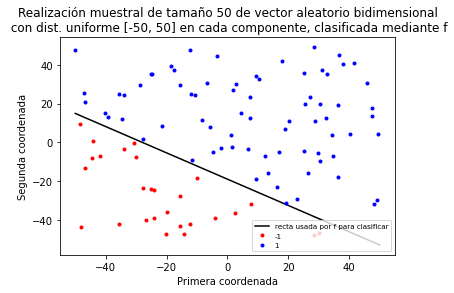
\includegraphics[width=0.66\textwidth]{images/1_2_a}
		\caption{Realización muestral de tamaño 50 de vector aleatorio bidimensional con distribución $U(-50,50)$ en cada componente.}
	\end{figure}
	%\textit{Nota:} en el código la función que clasifica la llamamos $f$ y ya incluye la función signo.\\
	donde se puede observar que todos los puntos están bien clasificados. Es decir, tenemos $Accuracy=1$ donde
	$$Accuracy:= \frac{TP + TN}{P + N}$$
	nos da la proporción de predicciones correctas (tanto positivas como negativas). Aquí \textit{TP} denota el número de predicciones positivas correctas, \textit{TN} el número de predicciones negativas correctas, \textit{P} el número verdadero de puntos con etiqueta positiva y \textit{N} el número verdadero de puntos con etiqueta negativa. Esta medida, $Accuracy$, no es más que $1-E_{in}(g)$, en este caso estamos evaluando $E_{in}(f)$ que es 0, por lo que $Accuracy=1-0=1$.\\
	
	Ahora simulamos ruido en el etiquetado, para ello se cambiará la etiqueta del 10\% de puntos con etiqueta +1 y del 10\% de puntos con etiqueta -1, en ambos casos los puntos se escogen de forma aleatoria. El resultado se puede visualizar en la siguiente gráfica:
	\begin{figure}[H]
		\centering
		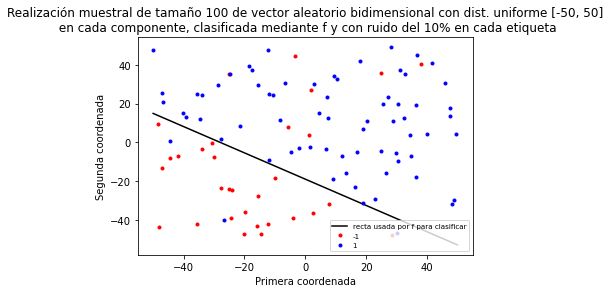
\includegraphics[width=0.9\textwidth]{images/1_2_b}
		\caption{Realización muestral de tamaño 100 de vector aleatorio bidimensional con distribución $U(-50,50)$ en cada componente, clasificada mediante $f$ y con ruido del 10\% en cada etiqueta.}
	\end{figure}
	en este caso obtenemos $Accuracy=0.9$
	
	Ahora vamos a comparar la clasificación que obteníamos mediante la recta con la que obtendríamos con diferentes funciones frontera de clasificación.
	
	\begin{itemize}
	
	\item $f(x,y)=(x-10)^2+(y-20)^2-400$ \ \ (elipse)
	\begin{figure}[H]
		\centering
		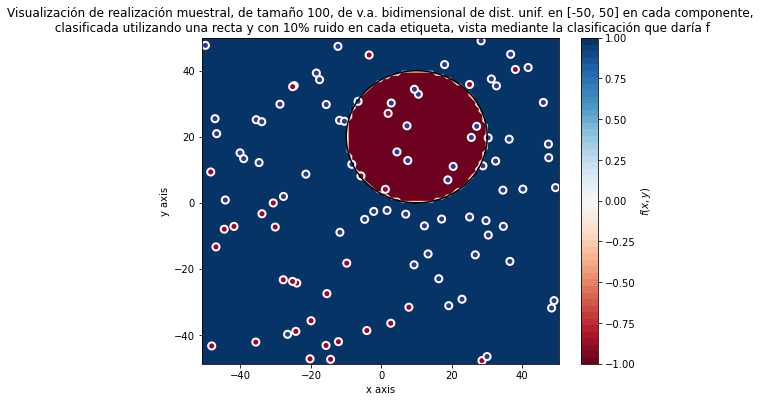
\includegraphics[width=0.92\textwidth]{images/1_2_c_f1}
		\caption{Visualización de realización muestral, de tamaño 100, de vector aleatorio bidimensional con distribución $U(-50,50)$ en cada componente, clasificada mediante recta y con 10\% de ruido en cada etiqueta. La visualizamos mediante la clasificación que nos daría la función frontera $f$}
	\end{figure}
	\item $f(x,y)=0.5(x+10)^2+(y-20)^2-400$ \ \ (elipse)
	\begin{figure}[H]
		\centering
		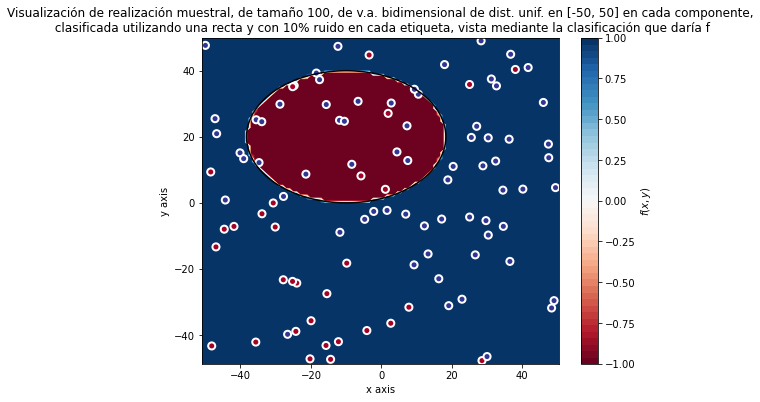
\includegraphics[width=0.92\textwidth]{images/1_2_c_f2}
		\caption{Visualización de realización muestral, de tamaño 100, de vector aleatorio bidimensional con distribución $U(-50,50)$ en cada componente, clasificada mediante recta y con 10\% de ruido en cada etiqueta. La visualizamos mediante la clasificación que nos daría la función frontera $f$}
	\end{figure}
	\item $f(x,y)=0.5(x-10)^2-(y+20)^2-400$ \ \ (hipérbola)
	\begin{figure}[H]
		\centering
		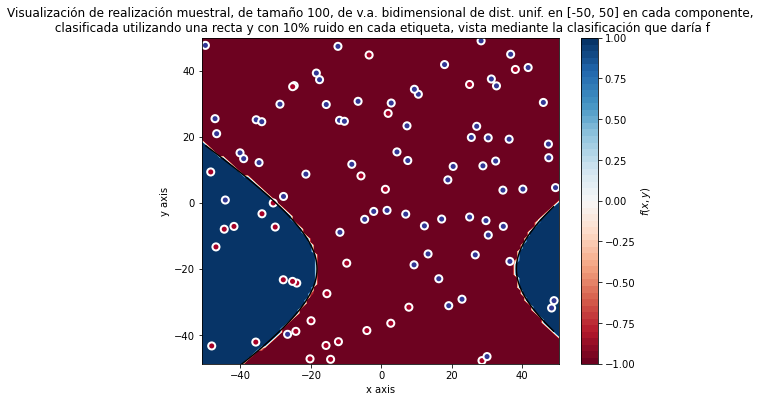
\includegraphics[width=0.92\textwidth]{images/1_2_c_f3}
		\caption{Visualización de realización muestral, de tamaño 100, de vector aleatorio bidimensional con distribución $U(-50,50)$ en cada componente, clasificada mediante recta y con 10\% de ruido en cada etiqueta. La visualizamos mediante la clasificación que nos daría la función frontera $f$}
	\end{figure}
	\item $f(x,y)=y-20x^2-5x+3$ \ \ (parábola)
	\begin{figure}[H]
		\centering
		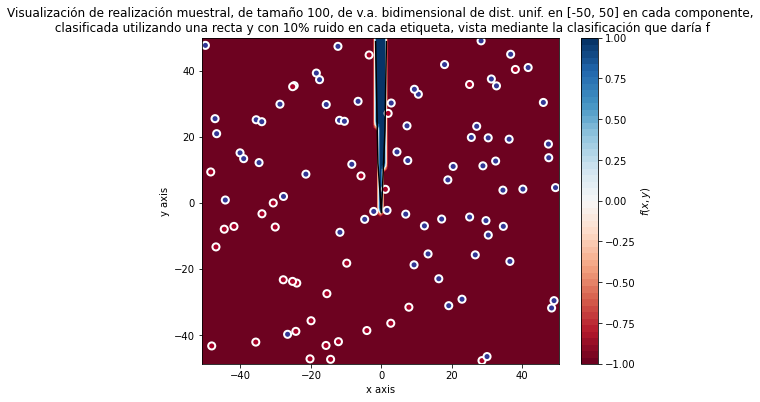
\includegraphics[width=0.92\textwidth]{images/1_2_c_f4}
		\caption{Visualización de realización muestral, de tamaño 100, de vector aleatorio bidimensional con distribución $U(-50,50)$ en cada componente, clasificada mediante recta y con 10\% de ruido en cada etiqueta. La visualizamos mediante la clasificación que nos daría la función frontera $f$}
	\end{figure}
	
	\end{itemize}
	
	A simple vista, ninguna de las nuevas funciones parece mejorar la clasificación que nos ofrecía la recta original. Para comprobar esto, hemos calculado de nuevo la medida $Accuracy$ para las diferentes funciones. \iffalse Para comprobar esto, como en principio no hay predilección por la clase -1 o +1, utilizaremos la medida
	$$Accuracy = \frac{TP + TN}{P + N}$$
	que nos da la proporción de predicciones correctas (tanto positivas como negativas). Aquí \textit{TP} denota el número de predicciones positivas correctas, \textit{TN} el número de predicciones negativas correctas, \textit{P} el número verdadero de puntos con etiqueta positiva y \textit{N} el número verdadero de puntos con etiqueta negativa.\fi
Llamando $f$ a la función original de clasificación, $f_1(x,y)=(x-10)^2+(y-20)^2-400$, $f_2(x,y)=0.5(x+10)^2+(y-20)^2-400$, $f_3(x,y)=0.5(x-10)^2-(y+20)^2-400$ y $f_4(x,y)=y-20x^2-5x+3$, tenemos la tabla:
	
	\begin{table}[H]
	\begin{center}
	\begin{tabular}{|c|c|c|}
	\hline
	Función frontera & Accuracy \\
	\hline \hline
	$f$ & 0.9 \\ \hline
	$f_1$ & 0.59\\ \hline
	$f_2$ & 0.51\\ \hline
	$f_3$ & 0.16\\  \hline
	$f_4$ & 0.27\\ \hline
	\end{tabular}
	\caption{Accuracy para distintas funciones frontera}
	\label{tabla:sencilla}
	\end{center}
	\end{table}
	Claramente, la función para clasificar que sigue ofreciendo mejor resultado, con accuracy 0.9, es $f$, la función original en la que utilizamos una recta para clasificar. Le siguen las elipses $f_1$ y $f_2$ con accuracy 0.59 y 0.51. Finalmente tenemos la parábola $f_4$ con accuracy 0.28, y con el peor resultado la hipérbola $f_3$ con accuracy 0.16; en estos dos últimos casos no llegamos ni siquiera a accuracy 0.5 que conseguiríamos en promedio con clasificador aleatorio.
	
	Por tanto, como generalmente el objetivo de utilizar funciones más complejas es disminuir el error dentro de la muestra a expensas de asumir mayor error de generalización (debe haber un equilibrio entre la complejidad de $\mathcal{H}$ y el error en la muestra), y sin embargo estamos consiguiendo mayor error en la muestra (menor accuracy); podemos concluir que estas nuevas funciones no son mejores clasificadores que la función lineal $f$.
	
	De todas formas, sabiendo que la función objetivo es una recta, no tiene sentido intentar elegir $\mathcal{H}$ con funciones más complejas para adaptarse al ruido. Muestras con ruido pueden sugerir funciones hipótesis más complejas cuando en realidad la función objetivo es simple; se debe evitar sobreajustar por ese ruido.
	
	
	%Muestras con ruido pueden sugerir funciones hipótesis más complejas cuando en realidad la función objetivo es simple. En nuestro caso, sabiendo que la función objetivo es lineal, no tiene sentido elegir funciones más complejas para adaptarse esta muestra con ruido. La clase de funciones, $\mathcal{H}$, no debe elegirse en base a la muestra, esto puede llevar un gran sobreajuste (menor error en la muestra pero mayor error de generalización).
	\iffalse , en nuestro caso una recta\fi %En nuestro caso, con $f_i$, $i=1,2,3,4$ no llegamos a disminuir el error en la muestra. Pero aunque hubiésemos elegido otras funciones con menor error en la muestra habría que valorar posteriormente el sobreajuste (menor error en la muestra pero mayor error de generalización) que conllevan.% Utilizar funciones hipótesis complejas puede dar lugar a sobreajuste (menor error en la muestra pero mayor error de generalización), en nuestro caso con $f_i$, $i=1,2,3,4$ no llegamos a disminuir el error en la muestra.
	%En el proceso de añadir ruido hemos obtenido una muestra sobre la que se ha decidido probar funciones hipótesis más complejas, esto no solo no ha conseguido disminuir el error en la muestra si no que también aumenta el error de generalización. 
    \newpage
    \section{Modelos Lineales.}
    \subsection{Apartado a)}
    El \textit{Algoritmo de Aprendizaje Perceptron} es caso particular del algoritmo \textit{Gradiente Descendente Estocástico} para tamaño minibatch 1 y tasa de aprendizaje 1 para la función $error(w^T x_n, y_n)=\max \{0, -y_n w^T x_n\}$, las funciones hipótesis tiene la forma $h_w(x)=sign(w^Tx)$ donde $x$ tiene 1 en la primera componente.
    La regla de adapación del algoritmo es 
		$$\begin{cases}
		w_{updated} = w_{current} +y_ix_i & sign(w^Tx_i) \neq y_i\\
		w_{updated} = w_{current} & sign(w^Tx_i) = y_i
		\end{cases} \quad \quad (*)$$
		es decir, teniendo un dataset $\mathcal{D}$ de tamaño $N$, $\mathcal{D}=\{(x_1,y_1),\ldots,(x_N,y_N)\}$, lo que hacemos es recorrerlo con $i=1,\ldots, N$ y actuar conforme (*) para cada $i$. Por lo que, si $x_i$ no está bien clasificado, entonces actualizamos el vector de pesos actual, $w$, en la dirección correcta; si está bien casificado no se hace nada. Estos recorridos del dataset siguiendo este criterio los repetimos hasta que se consiga un recorrido completo del dataset en el que no haya ningún punto mal clasificado.\\
		\textit{Nota:} si la muestra no es separable el algoritmo no llegará a clasificar correctamente toda la muestra, en este caso debe añadirse otra condición de parada, número máximo de épocas por ejemplo.
		%El algoritmo continuará hasta una condición de parada, ya sea por iteraciones o por haber clasificado correctamente toda la muestra (esto solo es posible si la muestra es separable).
		Se adjunta código de la implementación de PLA (autoexplicativo)
    \begin{lstlisting}[language=Python, caption= Implementaci\'on de algoritmo PLA en Python, inputencoding=latin1]
  '''
   Implementación de algoritmo PLA. 
   
   :param numpy.ndarray datos: matriz muestral de vectores de características con 1s en primera columna
   :param numpy.ndarray label: vector con etiquetas +1 o -1 de la muestra
   :param int max_iter: iteraciones o épocas máximas permitidas
   :param numpy.ndarray vini: valor inicial del vector de pesos
   :return: el último vector de pesos calculado y el número de iteraciones realizadas
'''
def ajusta_PLA(datos, label, max_iter, vini):
    
    w = vini.copy() # guardamos vector de pesos inicial
    wrong_class = True  # suponemos que existe al menos un punto mal clasificado
    it = 0 
    # Mientras no superemos el máximo de iteraciones y haya puntos mal clasificados
    while it < max_iter and wrong_class:
        wrong_class = False # suponemos que no hay puntos mal clasificados
        it += 1
        # Recorremos Dataset; vector caract con 1 al principio y la etiqueta asociada al v. características
        for x, y in zip(datos, label):
            # Si está mal clasificado
            if signo(x.dot(w)) != y:
                w = w + y * x # actualizamos vector pesos desplazando en la dirección correcta
                wrong_class = True # anotamos que había punto mal clasificado
        
    return w, it
	\end{lstlisting}
		Ejecutamos el algoritmo PLA con los datos simulados en partado 2a) de la sección anterior inicializando con el vector cero y, con vector de números aleatorios en [0,1], 10 veces en ambos casos. En ambos casos PLA convergerá a una solución ya que la muestra es separable. Mostramos los resultados.
		\begin{itemize}
			\item Vector de pesos inicial $(0,0,0)^T$. En este caso obtenemos una media de 75 iteraciones. Es más, obtenemos 75 iteraciones en las 10 repeticiones ya que estamos repitiendo bajo las mismas condiciones.\\ Podemos ver la recta obtenida en la última ejecución de PLA:
			\begin{figure}[H]
			\centering
			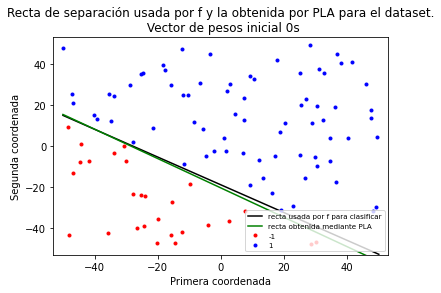
\includegraphics[width=0.6\textwidth]{images/pla_no_ruido_0s}
			\caption{Recta obtenida mediante PLA, con vector de pesos inicial de 0s, junto con la original. $Accuracy=1$}
			\end{figure}
			\item Vector de pesos inicial números aleatorios en [0,1]. Ahora obtenemos una media de 110.9 iteraciones (épocas), en concreto obtenemos el vector de iteraciones $[60, 248, 43, 72, 129, 244, 70, 84, 122, 37]$. Éstas van variando ya que en cada iteración el vector de pesos inicial es diferente.\\ Podemos ver la recta obtenida en la última ejecución de PLA:
			\begin{figure}[H]
			\centering
			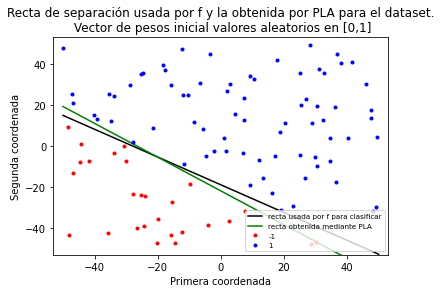
\includegraphics[width=0.6\textwidth]{images/pla_no_ruido_random_vals}
			\caption{Recta obtenida mediante PLA, con vector de pesos inicial conformado por valores aleatorios en $[0,1]$, junto con la recta original. $Accuracy=1$}
			\end{figure}
		\end{itemize}
		El algoritmo Perceptrón es sensible al punto inicial de pesos:
		\begin{itemize}
		\item Para la muestra con la que se ha trabajado el vector de pesos inicial $(0,0,0)^T$ toma menor número de épocas o iteraciones en converger, que el promedio de los vectores de pesos iniciales con valores aleatorios en [0,1]. La sensibilidad del vector inicial se puede observar en el vector de iteraciones del segundo caso, donde hay convergencia en 43 iteraciones con cierto punto inicial y con otro llega a necesitar hasta 248 iteraciones. El número de épocas que toma PLA depende de la proximidad de $w$ a una solución que separe la muestra, cuanto más cerca menos épocas.
		
		\item También podemos observar que con vector de pesos inicial $(0,0,0)^T$ obtenemos recta con pendiente más proxima a la que se utilizó para clasificar. Dependiendo del vector inicial de pesos también obtendremos mejores o peores soluciones. La solución se basa en la muestra y hay infinitas rectas que separan la muestra con $accuracy=1$, dependiendo del vector inicial de pesos se podrán obtener diferentes rectas. Un tamaño muestral $N$ grande evitaría esta variabilidad.
		\end{itemize}
		Ahora procedemos igual pero con la muestra con ruido, ya no será separable la muestra y no habrá convergencia. Mostramos los resultados.
		\begin{itemize}
			\item Vector de pesos inicial $(0,0,0)^T$. En este caso obtenemos 1000 iteraciones en todas las repeticiones, el algoritmo está parando por llegar al límite de iteraciones que tenía como argumento. No llega a una solución porque la muestra no es separable.\\ Podemos ver la recta obtenida en la última ejecución de PLA:
			\begin{figure}[H]
			\centering
			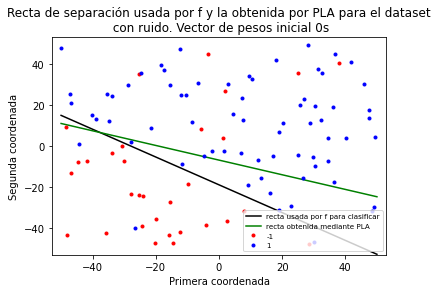
\includegraphics[width=0.6\textwidth]{images/pla_ruido_0s}
			\caption{Recta obtenida mediante PLA, con vector de pesos inicial de 0s, junto con la original. $Accuracy=0.91$}
			\end{figure}
			\item Vector de pesos inicial números aletorios en [0,1]. En este caso ocurre lo mismo, se obtiene 1000 iteraciones, el límite que se pasó como argumento, en todas las repeticiones ya que la muestra no es separable.\\ Podemos ver la recta obtenida en la última ejecución de PLA:
			\begin{figure}[H]
			\centering
			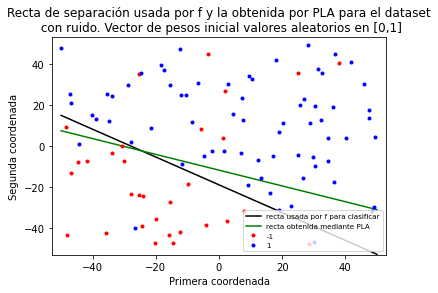
\includegraphics[width=0.6\textwidth]{images/pla_ruido_random_vals}
			\caption{Recta obtenida mediante PLA, con vector de pesos inicial conformado por valores aleatorios en $[0,1]$, junto con la recta original. $Accuracy=0.93$}
			\end{figure}
		\end{itemize}
    \subsection{Apartado b)}
    Dado un espacio probabilístico $(\Omega,\mathcal{A},P)$, suponemos vector aleatorio $\mathbf{x}=(x_1, x_2)\colon \Omega \to \R ^2$ con $x_1 \sim U(0,2)$, $x_2 \sim U(0,2)$, esto es, la distribución de probabilidad que inducen $x_1$ y $x_2$ siguen una distribución uniforme $U(0,2)$. Para obtener un dataset $\mathcal{D}$, realización muestral, de una muestra de $(\mathbf{x},y)$, $(\mathbf{x}_1,y_1),\ldots,(\mathbf{x}_N,y_N)$, elegiremos una recta en $\mathcal{X}=\mathbf{x}(\Omega)=[0,2]\times[0,2]$ que utilizaremos para clasificar la muestra, es decir, dar valores a variable aleatoria $y$, obteniendo así $y_1,\ldots,y_N$ \\
    \textit{Nota:} la clasificación se hará con etiquetas +1 y -1, $y(\Omega)=\{-1,+1\}$\\
    
    \underline{Método de Regresión Logística binaria:} \\%(suponemos ahhora vector aleatorio $x$ de dimensión $d$ y lo reescribimos como $x=(1,x_1,\ldots,x_d)$)\\
    Suponemos ahora caso general de $x=(x_1,\ldots,x_d)$ vector aleatorio de dimensión $d$. Sabemos que $P(x,y)=P(x)P(y|x)$. Regresión Logística binaria consiste en estimar $P(y|x)$ para luego clasificar asignando a la clase más probable (regla de Bayes).
    
    Si tomamos como función objetivo $f\colon \mathcal{X}\to [0,1]$ con $f(x)=P(y=1|x)$ y, reescribiendo $x=(1,x_1,\ldots,x_d)$,  como clase de funciones hipótesis
    $$\mathcal{H}:=\{h_w\colon \R^{d+1}\to \R \ :\ h_w(x)=\sigma(w^Tx),\ w \in \R^{d+1}\}$$
	donde $\sigma$ es la función logística (sigmoide), $\sigma\colon \R \to [0,1]$, $\sigma(x)=\frac{1}{1+e^{-x}}=\frac{e^x}{e^x+1}$
	\begin{figure}[H]
	\centering
	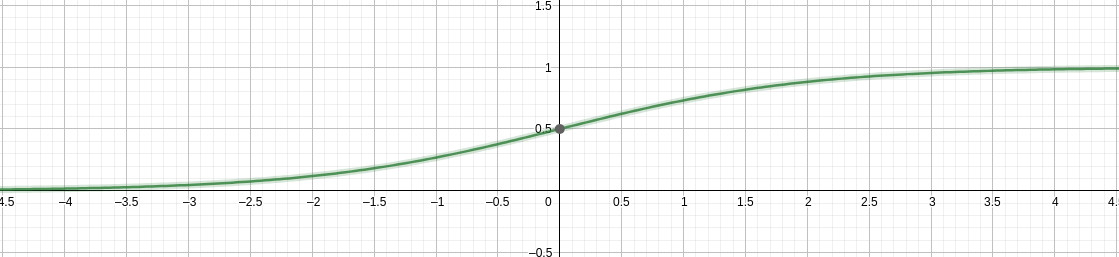
\includegraphics[width=0.6\textwidth]{images/sigmoide}
	\caption{Función sigmoide}
	\end{figure}
	tenemos que 
	$$ P(y| x) = \begin{cases} f(x) & y=+1 \\
	1-f(x) & y=-1
	\end{cases}$$
	y buscamos $h_w$ tal que 
	$$P(y| x)\approx \begin{cases} h_w(x) & y=+1\\
	1 - h_w(x) & y=-1
	\end{cases} \quad \quad (*)$$
	Podemos sustituir $h_w(x)$ por su valor, $\sigma(w^Tx)$, y utilizar que $1-\sigma(w^Tx)=\sigma(-w^Tx)$ para deducir que (*) equivale a  $P(y|x)\approx \sigma(yw^Tx)$\\
	
	\underline{Error en la muestra $E_{in}$ (\textit{maximum likelihood}):} En general, dada una muestra $(x_1,y_1),\ldots,(x_N, y_N)$ i.i.d, la probabilidad de obtener todos los $y_i$ correspondientes a los $x_i$ es
		$$\prod_{n=1}^N P(y_n | x_n)$$ 
		Supuesta esta muestra i.i.d. y una función hipótesis $h_w(x)=\sigma(w^Tx)$, queremos ver cómo de buena es $h_w$ para la muestra.
		
		Idea subyacente: ``Dada $h_w \in \mathcal H$, supogamos que $h_w=f$, ¿cuál sería la probabilidad de obtener la realización muestral, $(x_1,y_1),\ldots,(x_N, y_N)$, si mi hipótesis es cierta? Si es baja entonces nuestra $h_w$ no es muy buena, si la probabilidad es alta entonces $h_w$ sí es plausible''
		
		El método \textit{maximum likelihood} selecciona la función hipótesis $h_w$ que maximiza esta probabilidad vista como función de $w$, es decir queremos maximizar (recordar la equivalencia de (*) para lo siguiente)
	$$L(w)\iffalse=\prod_{i=1}^N P(y_i|x_i)\fi=\prod_{i=1}^N \sigma (y_i w^T x_i) $$
	Como $-\frac{1}{N} \ln()$ es decreciente, maximizar $L(w)$ equivale a minimizar 
		$$-\frac{1}{N} \ln\left( \prod_{n=1}^N \sigma(y_n w^T x_n)\right)=\frac{1}{N} \ln\left( \prod_{n=1}^N \frac{1}{\sigma(y_n w^T x_n)}\right)=\frac{1}{N}  \sum_{n=1}^N \ln \left( \frac{1}{\sigma(y_n w^T x_n)} \right)$$
		Sustituyendo la función sigmoide por su expresión, tenemos finalmente
		$$E_{in}(w):=\frac{1}{N} \sum_{n=1}^N \ln \left(1+e^{-y_nw^Tx_n}\right)$$
		%Si $e(h_w(x_n),y_n):=\ln (1+e^{-y_nw^T x_n})$, podemos ver que $e(h_w(x_n),y_n)$ es valor pequeño, y positivo siempre, cuando $y_iw^Tx_i$ es grande.\\
		
	\underline{Minimizando $E_{in}$}\\
	Vemos que 
	$$\nabla E_{in}(w)=\frac{\partial}{\partial w} \left( \frac{1}{N} \sum_{i=0}^N \ln (1+e^{-y_i w^T x_i})\right)=\frac{1}{N}\sum_{i=0}^N -y_ix_i \frac{e^{-y_i w^T x_i}}{1+e^{-y_iw^Tx_i}}=\frac{1}{N}\sum_{i=0}^N -y_ix_i\sigma(-y_iw^Tx_i)$$
	Para calcular el mínimo de $E_{in}(w)$ utilizamos \textit{SGD}\\
	
	Para el caso de regresión logística binaria, si hemos obtenido estimador máximo verosímil, $\sigma(w^Tx)$; si $ \sigma(w^Tx_i)\geq 0.5$, se asigna $y_i=1$ y en caso contrario $y_i=-1$. Además $\sigma(w^Tx)\geq 0.5 \Leftrightarrow w^Tx\geq 0$ y $\sigma(w^Tx)=0.5 \Leftrightarrow w^Tx= 0$, por lo que la frontera de clasificación la obtendremos cuando $w^Tx=0$. Para el caso planteado en este apartado, $d=2$,  $w^Tx=0$ nos dará la recta frontera de clasificación.\\
	
	Se adjunta código de la implementación de Regresión Logística utilizando SGD para minimizar $E_{in}$ (autoexplicativo), con tasa de aprendizaje 0.01, tamaño de minibatches 1 y con criterio de parada: distancia entre el vector de pesos de la época anterior y la actual menor que 0.01, $\norm{w(t-1)-w(t)}<0.01$, $t$ indica la época.
    \begin{lstlisting}[language=Python, caption= Implementaci\'on de algoritmo de Regresi\'on Log\'istica (SGD) en Python, inputencoding=latin1]
  '''
   Implementación de algoritmo de Regresión Logística (SGD). 
   
   :param numpy.ndarray X: matriz muestral de vectores de características con 1s en primera columna
   :param numpy.ndarray y: vector con etiquetas +1 o -1 de la muestra
   :param int max_epocas: épocas máximas permitidas
   :param float learning_rate: tasa de aprendizaje
   :param int minibatches_size: tamaño minibatches
   :param float e_crit_parada: criterio parada para la distancia entre el vector de pesos de una época y el v. pesos de la época anterior
   :return: el último vector de pesos calculado y el número de épocas hasta la finalización del algoritmo
'''
def sgdRL(X, y, max_epocas, learning_rate=0.01, minibatches_size=1, e_crit_parada=0.01):
    w = np.zeros(X.shape[1]) # vector de pesos inicial 0s
    wt = w # vector de pesos  inicial en la primera época 0s
    wt_1 = [np.inf for i in range(X.shape[1])] # vector de pesos en la época anterior, +inf por no haber época anterior y evitar condición parada
    sample_size = X.shape[0] # tamaño de muestra
    indexes = np.arange(sample_size) # trabajaremos con índices
    # Mezclamos aleatoriamente la muestra (trabajando con índices) por primera vez
    np.random.shuffle(indexes)
    # Marcamos el primer minibatch
    minibatch_init = 0
    minibatch_end = minibatch_init + minibatches_size
    epocas = 0 # contaremos las épocas
    
    # Mientras que no alcancemos el máximo de iteraciones y ||w(t-1)-w(t)|| no alcance la cota
    while epocas < max_epocas and np.linalg.norm(wt_1 - wt) >= e_crit_parada:
        # Se toma el minibatch actual
        minibatch = indexes[minibatch_init:minibatch_end]
        # Se calcula el vector pesos para el minibatch tomado (dando el 'paso de mayor profundidad' en el minibatch)
        w = w - learning_rate * grad_Ein_minibatch_RL(X[minibatch], y[minibatch], w)
        # Se avanza al siguiente minibatch
        minibatch_init += minibatches_size
        minibatch_end += minibatches_size
        # Si ya hemos iterado en todos los minibatches (hemos completado una época)
        if (minibatch_init >= sample_size):
            # actualizamos vectores de pesos de época actual y anterior
            wt_1 = wt
            wt = w
            epocas += 1 # incrementamos número de épocas
            # Mezclamos aleatoriamente muestra (trabajando con índices), generando así nuevos minibatches
            np.random.shuffle(indexes)
            # reestablecemos valores para empezar por primer minibatch
            minibatch_init = 0
            minibatch_end = minibatch_init + minibatches_size
            
    return wt, epocas
	\end{lstlisting}
	
	Obtenemos dataset $(\mathbf{x}_1,y_1),\ldots,(\mathbf{x}_{100},y_{100})$ donde $y_i$, $i=1,\ldots, 100$ son determinados por la recta frontera $ax+b$ generada mediante \texttt{simula\_recta([0,2])} que nos da $a=0.07148873686922362$, $b=0.5605073221826213$. Utilizamos $signo(y-ax-b)$ para clasificar.  %(que sería la función resultante de asignar la clase más probable después de estimar $P(y=+1|x)$)
	
	\begin{figure}[H]
		\centering
		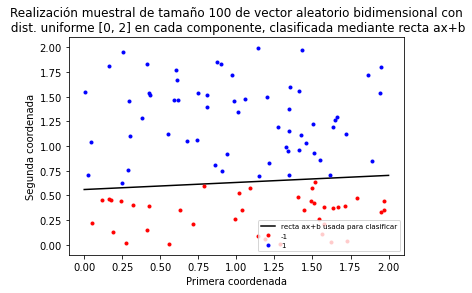
\includegraphics[width=0.7\textwidth]{images/rl1}
		\caption{Realización muestral de tamaño 100 de vector aleatorio bidimensional con distribución $U(0,2)$ en cada componente, clasificada mediante recta $ax+b$}
	\end{figure}
	Ejecutamos \texttt{sgdRL} con un máximo de 10000 épocas, después de 403 épocas el algoritmo encuentra solución y obtenemos vector de pesos $w=(-5.0760556, -0.70355299, 8.98142065)$, visualizamos la recta frontera estimada
	
	\begin{figure}[H]
		\centering
		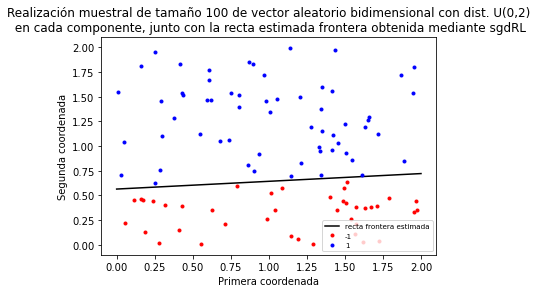
\includegraphics[width=0.7\textwidth]{images/rl2}
		\caption{Realización muestral de tamaño 100 vector aleatorio bidimensional con distribución $U(0,2)$ en cada componente, junto con la recta frontera estimada mediante la implementación de Regresión Logística (SGD). $Accuracy = 1$}
	\end{figure}
	Para la estimación, $g$, determinada por el vector de pesos obtenido $w$, tenemos
	\begin{itemize} 
		\item Error en la muestra $E_{in}(g)=0.09305945374997979$
		\item Una estimación del error fuera de la muestra, $E_{out}$, mediante $E_{test}$ para una muestra test de tamaño 1000, $E_{out}(g)\approx 0.08696362772944076$.
		\item La recta frontera separa la muestra de entrenamiento con $accuracy = 1$
		\item La recta frontera separa la muestra de test con $accuracy = 0.997$
	\end{itemize}
	Tenemos $0.08696\approx E_{test}(g)<E_{in}(g)\approx 0.09306$, siendo $E_{out}(g)\approx E_{test}(g)$ se puede decir se ha conseguido una función hipótesis buena, generaliza bien.\\
	Podemos visualizar la recta frontera obtenida junto con la original, bastante próximas, en la muestra test de tamaño 1000
	\begin{figure}[H]
		\centering
		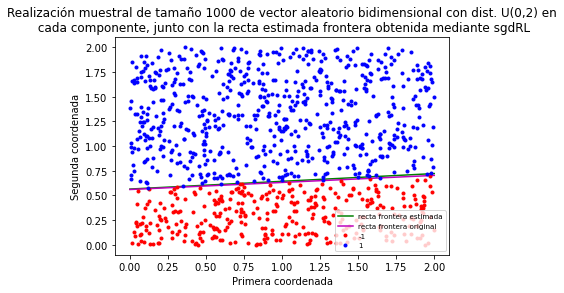
\includegraphics[width=0.8\textwidth]{images/rl_test}
		\caption{Realización muestral de tamaño 1000 de vector aleatorio bidimensional con distribución $U(0,2)$ en cada componente, junto con la recta estimada frontera obtenida mediante \texttt{sgdRL}.}
	\end{figure}
	
	\iffalse
	Repetimos el experimento 100 veces para obtener estimación promedio de $E_{out}$ y el promedio de épocas que toma el algoritmo en finalizar. Hemos obtenido:
	\begin{itemize}
		\item Promedio de estimaciones $E_{out}$ mediante $E_{test}$: $0.11531523104979062$. Este promedio de estimaciones de $E_{out}$ es algo mayor que el que obtuvimos en originalmente $\approx 0.08696$. No aporta mucha información esto, lo interesante es obtener cada par de error en la muestra y fuera de la muestra para ver si hay buena generalización.%; puede sugerirnos que obtuvimos muestra con bajo error.
		\item Promedio de épocas: $406.53$. Obtuvimos un número de épocas, 403, cercano al promedio. En el vector de épocas, excepto un par de casos más destacables en los que se obtuvieron 52 y 63 épocas, el resto están distribuidos entre 196 y 597 épocas. Hay variabilidad en el número de épocas requeridas por \texttt{sgdRL} en función de la muestra sobre la que se trabaje.
	\end{itemize}
	\fi
	Repetimos el experimento 100 veces, manteniendo la misma recta $ax+b$, para obtener estimación promedio de $E_{out}$ y el promedio de épocas que toma el algoritmo en finalizar. Hemos obtenido:
	\begin{itemize}
		\item Promedio de estimaciones $E_{out}$ mediante $E_{test}$: $0.10300234256866268$. Este promedio de estimaciones de $E_{out}$ es algo mayor que el que obtuvimos originalmente $\approx 0.08696$. Que el promedio de estimaciones difiera del estimación obtenida anteriormente muestra la variabilidad en las estimaciones, pues son estimaciones en base a una muestra test, cada muestra test da una estimación diferente (además, la función hipótesis elegida, $g$, depende de la muestra de entrenamiento, que también va variando).\\
		También se ha calculado el promedio de los errores en la muestra: 0.09220647539514909, valor cercano a las estimaciones de $E_{out}$. Por lo que, en promedio, tomar una realización muestral etiquetada o dataset y aplicar \texttt{sgdRL} (Regresión Logística (SGD)) proporciona una función hipótesis que generaliza bien.%Esto es, para 100 muestras de entrenamiento, se obtiene en promedio una estimación de $E_{out}$ algo superior a la obtenida original, aunque hay que tener en cuenta.Aún así se puede considerar que hay buena generalización. Que el promedio difiera del obtenido anteriormente muestra hay cierta variabilidad en las estimaciones, pues son estimaciones en base a una muestra test, cada muestra test da una estimación diferente.%; puede sugerirnos que obtuvimos muestra con bajo error.
		\item Promedio de épocas: $373.8$. Obtuvimos un número de épocas, 403, algo superior al promedio; en las 100 repeticiones del experimento el máximo de épocas fue 461 y el mínimo 307. Hay variabilidad en el número de épocas requeridas por \texttt{sgdRL} en función de la muestra de entrenamiento sobre la que se trabaje.
	\end{itemize}
	
	\newpage
	\section{Ejercicio Bonus.}
	\textbf{Planteamiento:} Suponemos $(\Omega,\mathcal{A},P)$ espacio probabilístico con $\Omega$ conjunto de todos los posibles dígitos manuscritos 4 y 8, $\mathcal{A}$ sigma álgebra de todos los subconjuntos posibles de $\Omega$, $P$ distribución de probabilidad desconocida. Tenemos las variables aleatorias $x_1\colon \Omega \to \R$ que mide la intensidad promedio (normalizada), $x_2\colon \Omega \to  \R$ que mide la simetría y $y\colon \Omega \to \R$ que asigna -1 si es 4 y +1 si es 8. Llamamos $\mathbf{x}$ al vector aleatorio $\mathbf{x}=(x_1,x_2)$. Tenemos $\mathcal{X}=\mathbf{x}(\Omega)=[0,1]\times \R$, $\mathcal{Y}=y(\Omega)=\{-1,1\}$\\
	\textit{Nota:} puede $x_2$, que mide la simetría, tenga un rango menor, habría que estudiar cómo está definida.
	
	Suponemos $(\mathbf{x}_1,y_1),\ldots,(\mathbf{x}_N,y_N)$ muestra aleatoria i.i.d (independiente idénticamente distribuida). Tenemos una realización muestral o dataset $\mathcal{D}=(\mathbf{x}_1,y_1),\ldots,(\mathbf{x}_N,y_N)$ (abuso de notación, ya no son vectores aleatorios). 
	
	Asumiendo que existe $f\colon \mathcal{X}\to \mathcal{Y}$ determinista, se busca una estimación $g$ de $f$, se utilizará criterio ERM, minimización del riesgo empírico, esto lo hacemos porque al ser la muestra i.i.d. podemos hacer uso de la desiguadad de Hoeffding generalizada a caso de $\mathcal{H}$ finita o infinita que nos asegura  $E_{out}(g)\approx E_{in}(g)$, si conseguimos $E_{in}(g)\approx 0 \Rightarrow E_{out}(g)\approx 0$ que es lo que buscamos. 
	
	La clase de funciones hipótesis en este caso es 
	$\mathcal{H}=\{h_w\colon \R^{3} \to \R \ : \ h_w(x) = sign(w^Tx), \ w \in \R^{3}\}$, se añade 1 en 1a componente a los vectores $\mathbf{x}_i,$ $i=1,\ldots,N$ del dataset ya que es más operativo. 
	
	La función de error a minimizar, la de clasificación, es
	$$E_{in}(h_w):=\frac{1}{N} \sum_{n=1}^N [[h_w(x)\neq y_n]]= \frac{1}{N} \sum_{n=1}^N [[sign(w^Tx_n)\neq y_n]] \quad \text{(proporción de puntos mal clasificados)}$$
	donde 
	$$[[sign(w^T x_n) \neq y_n]] = \begin{cases}
	1 & sign(w^T x_n)\neq y_n\\
	0 & sign(w^T x_n) = y_n
	\end{cases}
	$$
	indica 0 si con el vector de pesos $w$ clasificamos bien $x_n$ y 1 si clasificamos mal $x_n$.
	
	Sólo falta por determinar el algoritmo a utilizar.\\
	
	\textbf{Usar un modelo de Regresión Lineal y aplicar PLA-Pocket como mejora.}\\
	En regresión lineal la función de error es $$E_{in} (h_w):=\frac{1}{N}\sum_{i=1}^N(h_w(x_i)-y_i)^2$$
	por lo que realmente no minimiza el error adecuado para clasificación. Aún así, el vector de pesos que se obtenga, $w$, será un buen comienzo para el algoritmo de clasificación PLA-Pocket (que es el adecuado cuando la muestra no es separable como es nuestro caso).
	\begin{figure}[H]
		\centering
		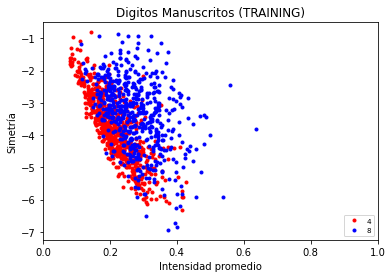
\includegraphics[width=0.6\textwidth]{images/bonus1}
		\caption{Muestra de entrenamiento. No separable}
	\end{figure}
	
	Elegimos método de Pseudoinversa, que nos proporciona analíticamente el mínimo y no una aproximación.
	
	Obtenemos el vector de pesos $w_{lin}=(-0.50676351,8.25119739, 0.44464113)$, podemos visualizar gráficamente la recta frontera obtenida en la muestra de entrenamiento
	\begin{figure}[H]
		\centering
		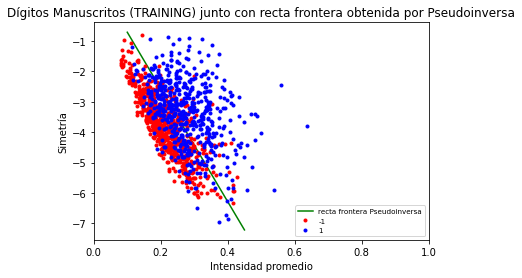
\includegraphics[width=0.8\textwidth]{images/bonus2}
		\caption{Muestra de entrenamiento junto con la recta frontera obtenida por Pseudoinversa}
	\end{figure}
	donde obtenemos $accuracy = 0.7721943048576214$, esto es, error de clasificación en la muestra $1-accuracy=0.22780569514237858=E_{in}(h_{w_{lin}})$. Para la muestra test
	\begin{figure}[H]
		\centering
		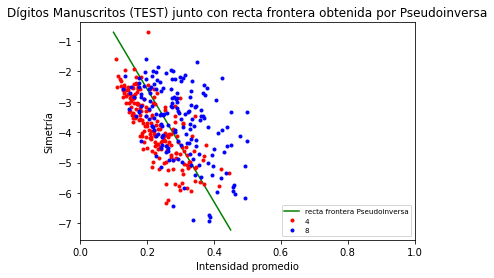
\includegraphics[width=0.8\textwidth]{images/bonus3}
		\caption{Muestra test junto con la recta frontera obtenida por Pseudoinversa}
	\end{figure}
	donde obtenemos $accuracy = 0.7486338797814208$, esto es, error de clasificación en la muestra test $1-accuracy=0.2513661202185792=E_{test}(h_{w_{lin}})$.\\
	
	Ahora aplicaremos PLA-Pocket partiendo del vector de pesos inicial obtenido mediante Pseudoinversa, $w_{lin}=(-0.50676351,8.25119739, 0.44464113)$. PLA-Pocket es PLA con dos distinciones: (1) no hay restricción de seguir mientras haya puntos mal clasificados, pues la idea es utilizarlo en muestras no separables, y (2) iremos anotando la mejor solución obtenida hasta el momento, la que proporcione menor error en la muestra. Al completar las épocas máximas indicadas se devolverá el vector de pesos óptimo.
	
	Se adjunta código de la implementación de PLA-Pocket (autoexplicativo)
	\begin{lstlisting}[language=Python, caption= Implementaci\'on de algoritmo PLA-Pocket en Python, inputencoding=latin1]
  #POCKET ALGORITHM
'''
   Implementación de algoritmo PLA-Pocket. 
   
   :param numpy.ndarray X: matriz muestral de vectores de características con 1s en primera columna
   :param numpy.ndarray y: vector con etiquetas +1 o -1 de la muestra
   :param numpy.ndarray w0: vector de pesos inicial
   :param int max_epocas: épocas máximas permitidas
   :return: vector de pesos óptimo calculado
'''
def PLA_Pocket(X, y, w0, max_epocas):
    w = w0.copy()
    w_opt = w.copy() # vector de pesos óptimo
    ep = 0 # controlamos el número de épocas
    # controlaremos el error óptimo
    err_opt = Ein_PLA_Pocket(X, y, w0) # asignamos error óptimo al obtenido con w0
    # Mientras no superemos el máximo de épocas permitidas
    while ep < max_epocas:
        # Recorremos dataset
        for x, et in zip(X, y):
            # Aplicamos criterio de adaptación de PLA
            if signo(x.dot(w)) != et:
                w = w + et * x
        # Evaluamos Ein(w) (error de clasificación en la muestra para v. pesos w) 
        ein = Ein_PLA_Pocket(X, y, w) # calculamos error que da w
        # Si el error en la muestra con w es menor que el óptimo hasta ahora
        if ein < err_opt:
            err_opt = ein # actualizamos error óptimo
            w_opt = w.copy() # guardamos el nuevo vector de pesos óptimo
        ep += 1 # incrementamos las épocas
        
    return w_opt
	\end{lstlisting}
	
	Después de la ejecución de PLA-Pocket obtenemos vector de pesos $\hat w= (-6.50676351, 94.33278003,\\ 4.88432863)$, error en la muestra de entrenamiento $0.22529313232830817$ y error en la muestra test $0.25409836065573765$. En la muestra de entrenamiento se ha obtenido un error menor que con Pseudoinversa que era lo que se buscaba. En la muestra test sin embargo se ha obtenido error algo mayor.
	
	\begin{figure}[H]
		\centering
		\begin{subfigure}{.5\textwidth}
  		\centering
  		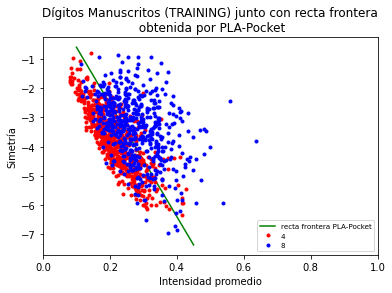
\includegraphics[width=1\textwidth]{images/bonus4}
  		\caption{Muestra entrenamiento}
  		\label{fig:sub1}
		\end{subfigure}%
		\begin{subfigure}{.5\textwidth}
  		\centering
  		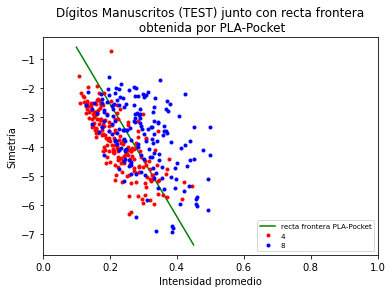
\includegraphics[width=1\textwidth]{images/bonus5}
  		\caption{Muestra test}
  		\label{fig:sub2}
		\end{subfigure}
		\caption{Rectas frontera obtenidas mediante PLA-Pocket}
		\label{fig:test}
	\end{figure}
	
	\textbf{Cotas de $E_{out}$:}\\
	Recordamos que a partir de la desigualdad de Hoeffding para caso de $\mathcal{H}$ finito
	$$P[ |E_{in}(g)-E_{out}(g)|>\epsilon]\leq 2 | \mathcal{H} | e^{-2\epsilon ^2N} \quad \forall \epsilon >0$$
	tomando $\delta =2|\mathcal{H}|e^{-2\epsilon ^2 N}$ y despejando $\epsilon$, tenemos
	$$E_{out}(g)\leq E_{in}(g)+\sqrt{\frac{1}{2N} \ln \frac{2|\mathcal{H}|}{\delta}}\quad \text{ con probabilidad } \geq 1-\delta$$
	
	\underline{Cota de $E_{out}$ basada en $E_{in}$:}\\
	En principio $\mathcal{H}=\{h_w\colon \R^{3} \to \R \ : \ h_w(x) = sign(w^Tx), \ w \in \R^{3}\}$ es infinito. Pero computacionalmente cada escalar tiene una representación de 64bits. Utilizando este hecho podemos obtener $\mathcal{H}$ finito. Como tenemos tres escalares $w\in \R^3$ $\Rightarrow$ podemos aproximar $|\mathcal{H}|\approx 2^{64}2^{64}2^{64}=2^{3\cdot 64}$. Nos queda 
	$$\quad E_{out}(h_{\hat w})\leq \underbrace{0.22529313232830817}_{E_{in}(h_{\hat w})} + \sqrt{\frac{1}{2\cdot 1194} \ln \frac{2\cdot 2^{3\cdot 64}}{0.05}} \quad \text{ con probabilidad } \geq 0.95$$
	esto es, $E_{out}(h_{\hat w})\leq 0.46461547451143265$ con probabilidad $\geq 0.95$\\
	
	\underline{Cota de $E_{out}$ basada en $E_{test}$:}\\
	En este caso hay que tener en cuenta que ya tenemos la función hipótesis fijada, $|\mathcal{H}|=|\{h_{\hat w}\}|=1$, por lo que 
	$$E_{out}(h_{\hat w})\leq \underbrace{0.25409836065573765}_{E_{test}(h_{\hat w})} + \sqrt{\frac{1}{2\cdot 366} \ln \frac{2}{0.05}} \quad \text{ con probabilidad } \geq 0.95$$
	esto es $E_{out}(h_{\hat w}) \leq 0.32508746408835315$ con probabilidad $\geq 0.95$. En este caso obtenemos mejor cota, más precisa, al tener $|\mathcal{H}|=1$
	
\end{document}
	

